\documentclass[11pt]{article}

\usepackage{tikz}
\usetikzlibrary{arrows.meta, positioning}
\usepackage[a4paper,margin=0.75in]{geometry}
\usepackage{enumitem}
\usepackage{hyperref}

\setlength{\parindent}{0pt}
\setlength{\parskip}{0.45em}
\setlist[itemize]{leftmargin=1.2em,itemsep=0.15em,topsep=0.15em}

\title{ARMv8 Group Project Final Report}
\author{Group 64: Rahul Babu, Rayan Abdallah, Ryan Wong, Ng Shi Hao}

\begin{document}
\maketitle

\section{Assembler Structure and Implementation}

We chose to use a two-pass assembler to assemble our code into a binary file since we found it to be relatively easier to implement as well as to split the work up between our group.

In the first pass, the source file is read to identify labels and record their instructions addresses in a symbol table to allow references to be resolved later during the second pass. In the second pass, each instruction or special directive is parsed into a 32-bit word and written to the output file in little-endian order. 

\texttt{assemble-file.c} uses a dispatch table to clearly identify which function needs to be called based on the given mnemonic. The functions to be chosen are parts of the data processing, data transfer, branch instructions and special directives. The functions that can be called are shown in the nodes in figure 1.

The assembler also handles aliases by translating them into a different form before parsing. For example, \texttt{cmp} is encoded as \texttt{subs} with the destination register set to the zero register, and \texttt{mul} is encoded as \texttt{madd} with the accumulate register set to the zero register. This reduced duplication and kept the encoding logic closer to the instruction formats.

The assembler was split and assigned to our different group members by different instruction types and handling of different passes through the code file. The first pass and file handling was implemented by Rayan, whereas the second pass was collaborated on by Rahul, Ryan and Rayan. A simplified architectural diagram of the assembler is in Figure 2. 

\section{Raspberry Pi LED Implementation}

Shi Hao and Ryan implemented an ARMv8 assembly program using the provided RPi kit to make the green LED blink. We controlled the LED using GPIO registers. 

The program loads the address of the function select register for pins 10-19, then configures GPIO17 as an output pin. It then enters an infinite loop labelled \texttt{blink}. In each iteration, it writes the GPIO17 bitmask to the set register. It creates a delay by using a large timing value and decrementing using \texttt{subs} and a conditional branch \texttt{b.ne}.

The constant definitions, such as the register addresses and bitmasks, are done using \texttt{.int} directives in order to make the program more readable and avoid the use of magic numbers, especially because hardware-specific values are even harder to understand.

The main challenge here was ensuring the GPIO pin was configured correctly before executing the main program logic. As the RPi does not give error output when the code does not run, debugging was challenging. To address this issue, we inspected file size and incrementally debugged the program: first ensuring that the GPIO 17 was configured correctly, then checking that it could be set and cleared, and finally fine-tuning the wait time to make the blinking behaviour observable.

\section{Extension: RackInsert-C}

Ryan and Shi Hao initially wanted to build a more ambitious robotics project involving Shi Hao's SO-101 robotic arms assembling Lego structures. However, w realised very quickly that this is unrealistic given full sim-to-real transfer, policy training, etc. is unfeasible given this project's timeline. Hence, we scoped the extension down to an evaluator/benchmark for robotics cable rack insertion (cable management is deemed as a challenging open problem in robotics). The structure of our code is inspired by Intrinsic AIC, a robotics competition Shi Hao attended earlier this year).\footnote{\url{https://www.intrinsic.ai/events/ai-for-industry-challenge}}

The benchmark and evaluator is written in C and split into modules: 

\begin{itemize}
    \item \texttt{sim.c}: Manages the core MuJoCo physics environment, scene loading, simulation reset logic, physics stepping, and robotic arm's actuator command execution.
    \item \texttt{scripted\_policy.c}: Implements the finite-state machine (FSM) controller, driving the robot across a series of smoothly interpolated, joint-space waypoints.
    \item \texttt{benchmark.c}: Orchestrates the execution of insertion trials and aggregates overall rollout statistics, including simulation duration and total path length.
    \item \texttt{evaluator.c}: Utilises vector algebra to compute precise spatial relationships between the plug and socket, translating these geometric metrics into a tiered evaluation score.
    \item \texttt{logging.c}: Generates terminal-based trial summaries and serializes millisecond-level trajectory telemetry to CSV files for post-trial replay and analysis.
\end{itemize}
The robot controller is a finite-state machine with four stages: \texttt{APPROACH}, \texttt{HOVER}, \texttt{ALIGN}, and \texttt{INSERT}. Each stage uses hard-coded joint-space offsets from the robot's home pose, hand-tuned by visual inspection until the rollout behaved reasonably. Rather than implementing inverse kinematics or a learned policy, joint commands are smoothly interpolated between stages to produce a stable baseline rollout.

The evaluator reads key MuJoCo sites, specifically \texttt{plug\_tip}, \texttt{socket\_mouth}, and \texttt{socket\_bottom}. From these, it computes plug-to-socket distance, lateral error from the socket axis, axial insertion depth, rollout duration, and plug-tip path length. These values are combined into a tiered score covering program validity, motion quality, and insertion success, turning a visual robotics task into numerical benchmark metrics.

The benchmark can also record CSV traces of rollouts, including joint states, actuator commands, plug-tip positions, and evaluation metrics over time. These traces can be replayed using a small Python script. The simulator, controller, benchmark, evaluator, logging, and tests are written in C; Python is only used for replay visualisation, since implementing a full C/GLFW MuJoCo viewer was outside the remaining project scope.

\section{Testing}

We tested the assembler using the provided ARMv8 test suite. These tests compare the binary output generated by our assembler against the expected binary output for a range of assembly programs. We tested individual instructions while developing, then ran the full assembler test suite once the components were integrated.

We also used more focused tests for instructions and instruction types. For example, \texttt{add}, \texttt{sub}, \texttt{movz}, branch, and load/store programs were tested individually. This helped isolate whether failures came from parsing, field placement, alias handling, endianness, or symbol resolution.

We believe we could have spent more time testing against invalid instructions. Invalid operand counts, shift amounts, register prefixes or unknown mnemonics. We did enforce checks for these within our program and created dedicated helper functions but more tests would have made our emulator even more robust.

For the extension, we wrote three main C test files. \texttt{test\_evaluator} follows a more conventional unit-test style, checking that the geometric calculations and scoring rules behave correctly for controlled plug/socket positions. However, \texttt{test\_actuators} and \texttt{test\_scripted\_policy} are closer to smoke tests, because actuator control and finite-state robot motion are difficult to validate with simple input-output assertions. These tests check that the MuJoCo scene loads successfully, actuator commands produce robot motion, and the scripted policy completes a rollout without timing out or leaving the plug stationary.

Visual testing through the MuJoCo GUI was also important, since many simulation bugs are easiest to diagnose by watching the robot move. This helped catch several issues that would not have been obvious from terminal output alone, such as incorrect initial robot positioning causing unstable jittering, and actuator definitions that did not produce stable control behaviour. In particular, testing the actuator pipeline helped us identify scene/control problems and move towards more stable position-based actuation. Although this testing approach is less conventional than pure unit testing, it was effective for validating a robotics simulation where the main failure modes involve physical behaviour over time.

\section{Group Reflection}

Overall, we split the work by project components and took design steps which made the implementation manageable and easier to divide between group members. Good use of Git made working in a team easier. For example, committing small amounts of code often, using \texttt{git pull} frequently, and working in individual branches helped reduce integration issues.

Our communication was best when work was clearly divided between team members. For example, assigning Rayan to part 2.1 and 2.2, Rahul to Part 2.3.1 and Ryan Wong to Parts 2.3.2 to 2.3.4 made ownership clearer. However, one issue was that some modules depended on parsing variations, universal constants, and use of the symbol table, so care had to be taken to communicate proposed changes to each other, especially when our common standards were affected. We believe that our distribution of work was acceptable to all. We would have benefitted from agreeing on naming conventions, shared interfaces and function design before starting implementation on overlapping aspects, as well as being more proactive in communicating.

\section{Individual Reflections}

\subsection{Rahul}
I worked on the data processing assembler implementation. My main strength was breaking the instruction formats down into smaller cases and understanding how aliases mapped onto real encodings. I found one weakness to be that I needed some time to understand how the data processing parsing should be split across multiple functions and across multiple files. In a future group project, I will try to design earlier to ensure that future code refactoring would not take up too much time and effort. Furthermore, I would try to stick to code design principles earlier, such as better use of helper functions to avoid large blocks of repeated code.

\subsection{Rayan}
Overall I think our biggest mistake was not planning the full code together. I thought it’d have been a good idea to split up the spec into smaller chunks we each complete, but instead we should have all gone through and understood the full spec in a more complete way, as this would have helped us catch compatibility issues between our files later on. This also led us to having to change our peers’ code quite frequently near the end. Another thing to add is that we should have created our own sample tests for each of our sections, instead we relied on the provided tests and only used them once we had all completed the code, therefore if someone is late in finishing their portion of work it would result in all of us being delayed on the job. I thought my proficiency in C++ would’ve made it easier for me to write C but the lack of many libraries that aren’t available forced me to stick to the provided methods in lectures and to re-learn different ways of handling data issues. I wish I had started on the slides and report earlier too as including problems we faced while we were debugging and changing our plans could have saved us time and increased the valuable insights we may have forgotten later on.


\subsection{Ryan Wong}
Being in charge of the overall debugging effort for the assembler taught me the importance of discipline. As we divided the work on the assembler into disjoint sections, we each came up with different versions of register and hexadecimal parsing. Looking back, it would have been much easier to write and debug our code if we had proactively flagged potential duplications of work, discussed them in the group chat or in-person, and enforced a maximum lifespan of each separate branch to limit divergence from the master branch. 

While I feel I did a good job in facilitating discussions and distributing the work, my weakness lay in avoided friction too often. In hindsight, I should have been insistent about maintaining a bird's eye view of the project and more proactive in harmonizing our respective branches. The lengthy debugging process taught me the hard way to create standards early, embracing the friction generated from discussions. Overall, I learnt that clean, maintainable code is forged by the uncompromising commitment to coding the right way.


\subsection{Shi Hao}
My main responsibilities were the extension and part of the Raspberry Pi LED task. Looking back, I think our group improved significantly compared with the interim checkpoint, especially in reducing duplicated code and communicating more clearly around shared modules. However, I still think we could have planned interfaces and utility functions earlier. In particular, agreeing sooner on shared helper files and common abstractions would have made integration smoother and reduced the amount of refactoring needed.

For the extension, I am happy with how much I learned from building \texttt{RackInsert-C}. Before this project, most of my robotics experience was through Python/PyTorch workflows using simulators such as Isaac Sim, Gazebo, and MuJoCo, usually from the policy training side. This was my first time working directly with MuJoCo's C API and thinking more carefully about the upstream simulation infrastructure: loading scenes, controlling actuators, defining benchmark metrics, recording trajectories, and designing an evaluator. Even though we did not have time to implement the more ambitious goals, such as teleoperation and training an Action Chunking Transformer from recorded data, the final extension gave me a much clearer understanding of how robotics simulation environments are built underneath the higher-level tooling.

A particularly useful insight was seeing how similar robotics simulation infrastructure feels to other engineering simulation tools, such as finite element or fluid simulation software. In all cases, a large part of the work is not just the final model or controller, but designing the environment, defining meaningful measurements, and ensuring that the simulation can be run and evaluated reliably. In a future project, I would scope the learning-policy component more conservatively from the start. I would first make sure the simulator, evaluator, and data-recording pipeline are stable before adding more ambitious control methods.

\section{Appendix}

\pagebreak

\begin{figure}[h]
\centering
\resizebox{\textwidth}{!}{%
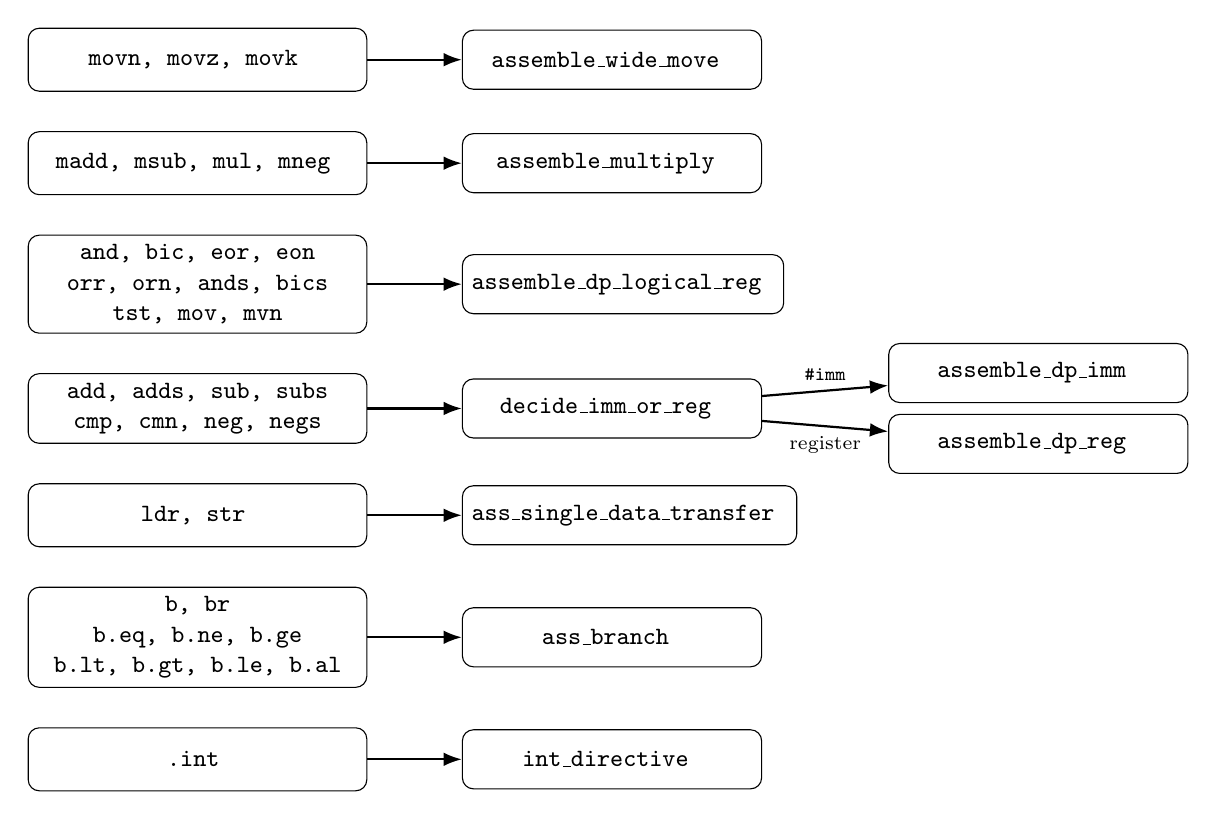
\begin{tikzpicture}[
    node distance=0.5cm and 1.2cm,
    mnemonic/.style={
        rectangle,
        draw,
        rounded corners,
        align=center,
        minimum width=4.3cm,
        minimum height=0.8cm,
        font=\small
    },
    function/.style={
        rectangle,
        draw,
        rounded corners,
        align=center,
        minimum width=3.8cm,
        minimum height=0.75cm,
        font=\small\ttfamily
    },
    arrow/.style={-Latex, thick}
]

\node[mnemonic] (wide_mnems) {
\texttt{movn, movz, movk}
};
\node[function, right=of wide_mnems] (wide_func) {
assemble\_wide\_move
};

\node[mnemonic, below=of wide_mnems] (mul_mnems) {
\texttt{madd, msub, mul, mneg}
};
\node[function, right=of mul_mnems] (mul_func) {
assemble\_multiply
};

\node[mnemonic, below=of mul_mnems] (logic_mnems) {
\texttt{and, bic, eor, eon}\\
\texttt{orr, orn, ands, bics}\\
\texttt{tst, mov, mvn}
};
\node[function, right=of logic_mnems] (logic_func) {
assemble\_dp\_logical\_reg
};

\node[mnemonic, below=of logic_mnems] (arith_mnems) {
\texttt{add, adds, sub, subs}\\
\texttt{cmp, cmn, neg, negs}
};
\node[function, right=of arith_mnems] (decide_func) {
decide\_imm\_or\_reg
};

\node[function, right=1.6cm of decide_func, yshift=0.45cm] (imm_func) {
assemble\_dp\_imm
};
\node[function, right=1.6cm of decide_func, yshift=-0.45cm] (reg_func) {
assemble\_dp\_reg
};

\node[mnemonic, below=of arith_mnems] (transfer_mnems) {
\texttt{ldr, str}
};
\node[function, right=of transfer_mnems] (transfer_func) {
ass\_single\_data\_transfer
};

\node[mnemonic, below=of transfer_mnems] (branch_mnems) {
\texttt{b, br}\\
\texttt{b.eq, b.ne, b.ge}\\
\texttt{b.lt, b.gt, b.le, b.al}
};
\node[function, right=of branch_mnems] (branch_func) {
ass\_branch
};

\node[mnemonic, below=of branch_mnems] (directive_mnems) {
\texttt{.int}
};
\node[function, right=of directive_mnems] (directive_func) {
int\_directive
};

\draw[arrow] (wide_mnems) -- (wide_func);
\draw[arrow] (mul_mnems) -- (mul_func);
\draw[arrow] (logic_mnems) -- (logic_func);
\draw[arrow] (arith_mnems) -- (decide_func);
\draw[arrow] (decide_func) -- node[above, font=\scriptsize] {\texttt{\#imm}} (imm_func);
\draw[arrow] (decide_func) -- node[below, font=\scriptsize] {register} (reg_func);
\draw[arrow] (transfer_mnems) -- (transfer_func);
\draw[arrow] (branch_mnems) -- (branch_func);
\draw[arrow] (directive_mnems) -- (directive_func);

\end{tikzpicture}
}
\caption{Assembler dispatch table mapping mnemonics to encoding functions.}
\label{fig:assembler-dispatch}
\end{figure}

\begin{figure}[ht]
\centering
\resizebox{\textwidth}{!}{%
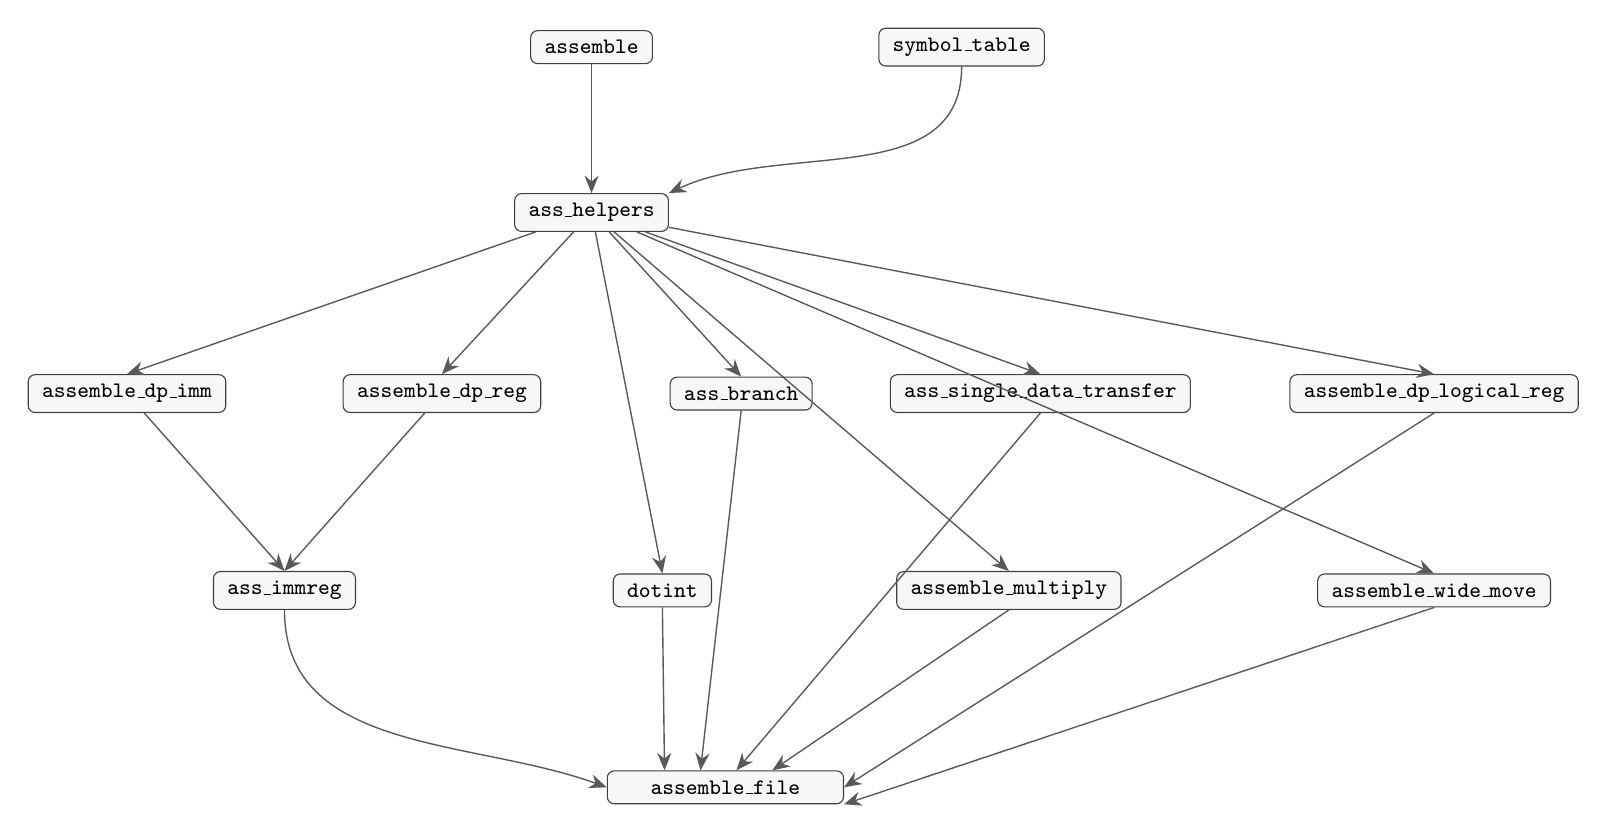
\begin{tikzpicture}[
    >={Stealth[length=2.2mm,width=1.8mm]},
    font=\ttfamily\footnotesize,
    box/.style={
        draw=black!75, rounded corners=2.5pt, align=center,
        inner xsep=5pt, inner ysep=3.5pt, fill=gray!6, line width=0.4pt
    },
    arr/.style={->, draw=black!65, line width=0.5pt},
]
% ---------- Layer 0 : entry points ----------
\node[box] (assemble) at (5.3, 0)  {assemble};
\node[box] (symtab)   at (10.0, 0) {symbol\_table};
% ---------- Layer 1 : dispatch hub ----------
\node[box] (helpers)  at (5.3, -2.1) {ass\_helpers};
% ---------- Layer 2 : per-instruction encoders ----------
\node[box] (dpimm)  at (-0.6, -4.4) {assemble\_dp\_imm};
\node[box] (dpreg)  at ( 3.4, -4.4) {assemble\_dp\_reg};
\node[box] (branch) at ( 7.2, -4.4) {ass\_branch};
\node[box] (sdt)    at (11.0, -4.4) {ass\_single\_data\_transfer};
\node[box] (dplog)  at (16.0, -4.4) {assemble\_dp\_logical\_reg};
% ---------- Layer 3 : leaf helpers ----------
\node[box] (immreg)  at ( 1.4, -6.9) {ass\_immreg};
\node[box] (dotint)  at ( 6.2, -6.9) {dotint};
\node[box] (mult)   at (10.6, -6.9) {assemble\_multiply};
\node[box] (wide)   at (16.0, -6.9) {assemble\_wide\_move};
% ---------- Layer 4 : output sink ----------
\node[box, minimum width=3cm] (file) at (7.0, -9.4) {assemble\_file};
% ===================== EDGES =====================
\draw[arr] (assemble) -- (helpers);
\draw[arr] (symtab.south) to[out=-90, in=25] (helpers.north east);
\draw[arr] (helpers) -- (dpimm.north);
\draw[arr] (helpers) -- (dpreg.north);
\draw[arr] (helpers) -- (branch.north);
\draw[arr] (helpers) -- (sdt.north);
\draw[arr] (helpers) -- (dplog.north);
\draw[arr] (helpers) -- (dotint.north);
\draw[arr] (helpers) -- (mult.north);
\draw[arr] (helpers) -- (wide.north);
\draw[arr] (dpimm) -- (immreg.north);
\draw[arr] (dpreg) -- (immreg.north);
% leaf helpers -> assemble_file (straight lines to distinct points on the top edge)
\draw[arr] (immreg.south) to[out=-90, in=160] (file.west);
\draw[arr] (dotint.south) -- ([xshift=-22pt]file.north);
\draw[arr] (branch.south) -- ([xshift=-9pt]file.north);
\draw[arr] (mult.south)   -- ([xshift=17pt]file.north);
\draw[arr] (sdt.south)    -- ([xshift=4pt]file.north);
\draw[arr] (dplog.south)  -- (file.east);
\draw[arr] (wide.south)   -- (file.south east);
\end{tikzpicture}%
}
\caption{Simplified dependency graph of the assembler. Helper functions include:
(1)~\texttt{parse\_reg}, which returns a register number while writing the size
flag, rejecting malformed tokens; and (2)~\texttt{read\_number\_or\_label}, which
resolves an operand that is either a label name, a hexadecimal literal, or a
binary literal, rejecting malformed operands.}
\label{fig:assembler-deps}
\end{figure}


\section{Extension Supplementary Material}

\subsection{Example Usage}

\begin{verbatim}
cd extension
make deps
make all
./rack_insert --trials 10 --trace results.csv
.venv/bin/python scripts/replay_trace.py --trace results.csv
\end{verbatim}

\subsection{MuJoCo Scene}

\begin{figure}[h]
    \centering
    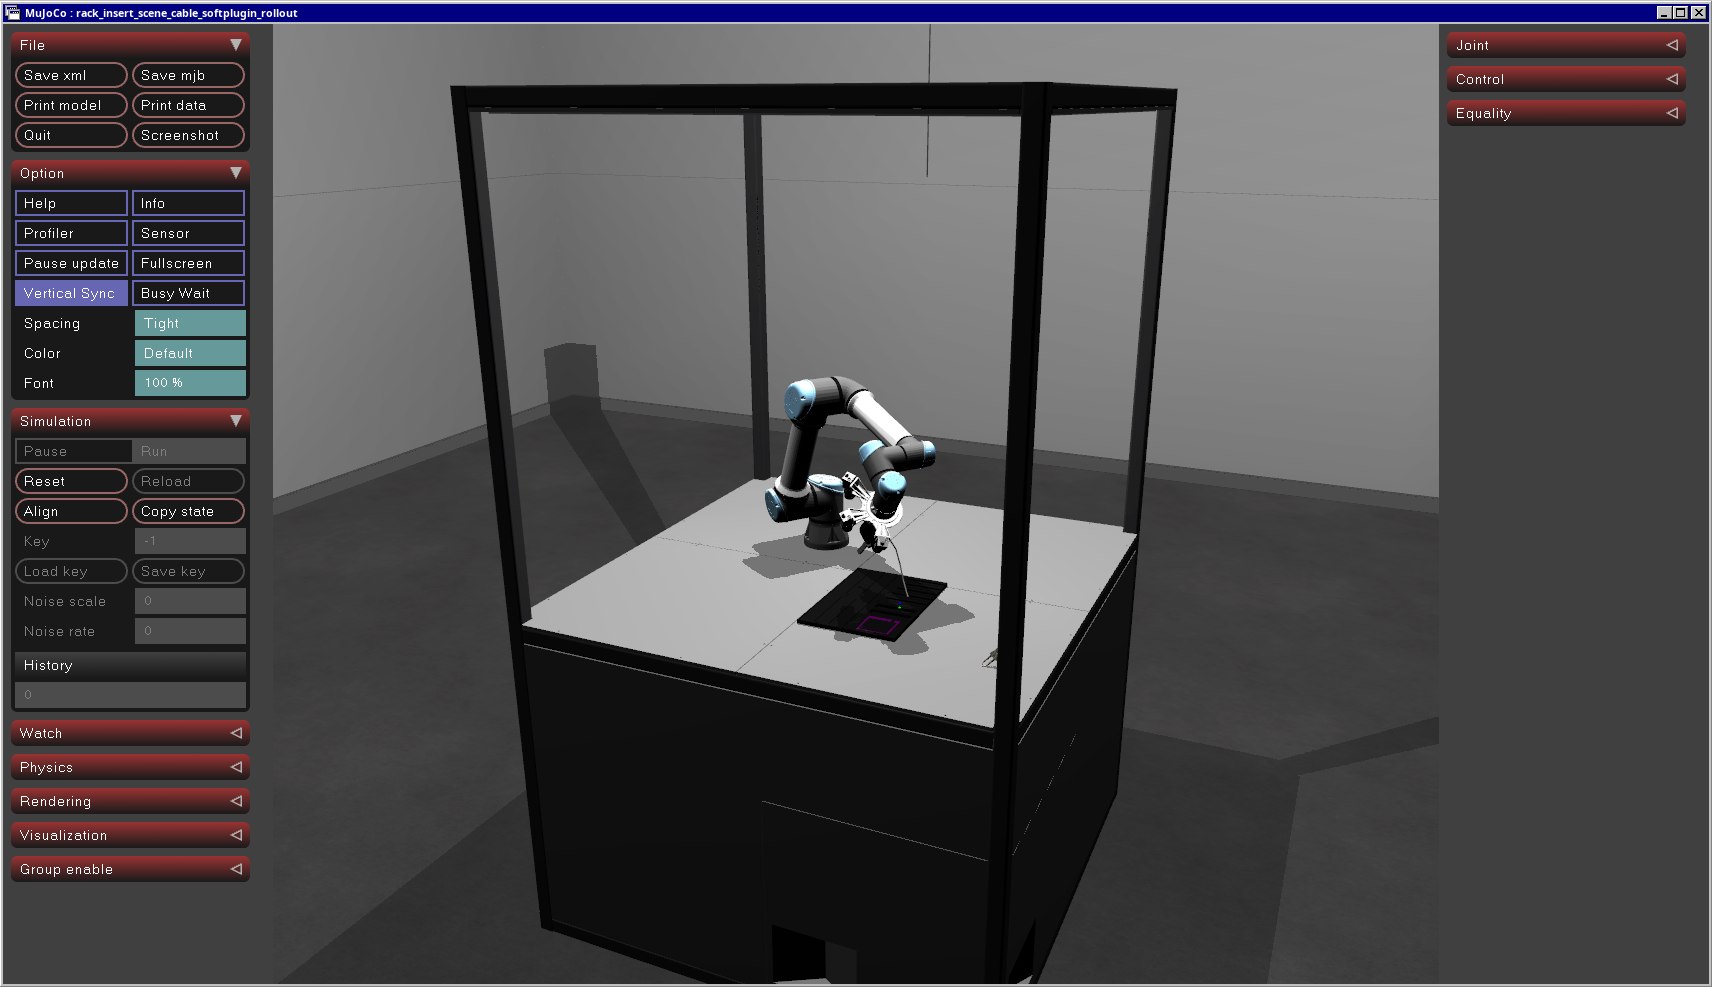
\includegraphics[width=0.75\linewidth]{mujoco-c.png}
    \caption{MuJoCo rack insertion scene used by the extension. The benchmark evaluates the plug tip position relative to the socket mouth and socket bottom.}
    \label{fig:mujoco-rack-insert}
\end{figure}

\subsection{Scene Assets and Design Rationale}

The rack-insertion task and scene assets are based on Intrinsic's AI for Industry Challenge, which focuses on robotic cable handling and connector insertion in electronics assembly. We chose this task because cable insertion is a difficult contact-rich robotics problem requiring precise alignment and controlled motion. Designing our own robot model, server rack, plug, socket, and collision geometry from scratch would have required substantial CAD and asset conversion work, so we instead focused our implementation effort on the C simulation wrapper, controller, benchmark loop, trace logging, and scoring pipeline.

The scene is represented using MuJoCo XML/MJCF assets. Working with these assets was still a significant part of the extension, since the C code had to reliably load MuJoCo plugins, find named joints and sites, command actuators, and extract 3D positions for evaluation.

\end{document}